\chapter{Introduction for Non-physicists}

One of the primary tenets of science is to communicate results to as wide an audience as possible.
But in this regard, dissertations can be funny things, as they tend to have the smallest audiences.
For physicists, the results that make up this dissertation either A) have been already communicated to the physics community through publications in journals and/or B) will be outdated within a year or two (such is progress).
For everyone else, I am sure it's just incomprehensible.

This introduction is my attempt to include the latter group and share with others, particularly family and friends, what I have been doing for the last five years.
So bear with me, as I try to condense the next $\sim$100 pages into this short introduction.
So, here goes...

The job of physcicists is to model how the universe works.
For particle physicists, in particular, we do this by understanding how fundamental particles interact with each other.
This gives us really profound insights into the universe as these particles and their interactions are the building blocks for the universe.
A ``fundamental particle'' is any particle that is not made up of smaller particles.
For example, neutrons and protons are not fundamental particles, as they are each composed of three ``quarks'', but an electron, on the other hand, is fundamental, as it is not made up of any smaller particles. 

There are two groups of fundamental particles: fermions and bosons.
Fermions are the particles that make up matter and combine to form protons and neutrons (as mentioned above) and eventually atoms, molecules, etc.
Bosons are the ``force carrier'' particles.
They allow the particles to interact with each other and are responsible for transferring forces between them.
For example, the photon mediates the electromagnetic force, i.e. electricity and magnetism.
The gluon is responsible for the ``strong force'', which is what holds atoms together, and the W and Z bosons carry the ``weak force'', which is what causes atoms to decay.
In total there are 12 fermions and 5 bosons, shown in Figure~\ref{fig:sm_particles}, that have been discovered so far.

Additionally, there are rules for which particles can interact with which particles and through which forces and with what strength, etc.
These rules are what particle physicicts work to study and attempt to model.
Our best understanding of these rules have been combined into the Standard Model of Particle Physics.
The Standard Model has been one of the greatest achievements of science.
It has been able to predict and explain a wide variety of phenomena and has withstood a number of stress tests.
To do this day, it is the most precisely tested theory in physics, if not science as a whole.

It wasn't until 2012, however, after almost 50 years of searching, that the Standard Model was completed with the discovery of the Higgs boson.
The Higgs boson was initially theorized in the 1960's and is the particle responsible for explaining why things have mass -- very succinctly, the amount a particle interacts with the Higgs boson is proportional to the amount of mass it has.
This was a profound discovery, and it showcased the incredible predictive power of the Standard Model, resulting in a Nobel prize and even making it to the front page of the New York Times, as shown in Figure~\ref{fig:nyt_higgs}.

\begin{figure}[tbp!]
\begin{center}
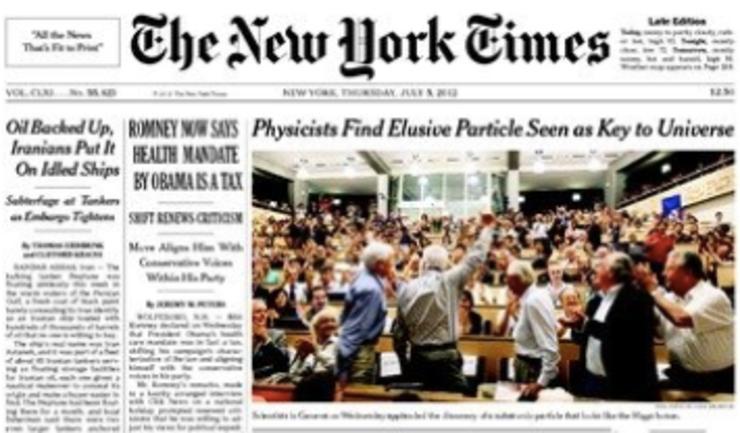
\includegraphics[angle=0,width=0.60\columnwidth]{fig/nyt_higgs.pdf}
\end{center}
\caption{The discovery of the Higgs boson made the front page of many newspapers, including the New York Times.}
\label{fig:nyt_higgs}
\end{figure}

There was, however, a downside to this discovery -- the Standard Model was completed.
Despite all the successes of the Standard Model, there are certain things we simply cannot explain with it.
For example, you may have noticed earlier that when I described the fundamental forces, I did not mention gravity.
This is because it turns out it's really, really difficult to combine the Standard Model and Einstein's theory of general relativity, which is our best description of gravity.
Furthermore, from astronomical measurements, we know there is something called Dark Matter and that it comprises 4x more of the matter in the universe than do the Standard Model particles, but we can't really say much more about it.
What this means is that the Standard Model cannot tell the full story of how the universe behaves and that there must be more undiscovered particles to fill in the gaps.

If we had not discovered the Higgs boson, it would have been a major clue to what the missing particles might be. 
Instead, we just have to be a bit more clever.
One way to get hints for what this new physics make look like is by examining where the Standard Model breaks down.
When you do the mathematical calculation of the Higgs boson mass, you get something close to infinity, while the measured mass of the Higgs boson is $125~\GeV/c^2$ (the units are unimportant here).
Clearly, there is a discrepancy.
One way to reconcile this difference with the Standard Model is if two independent parameters were perfectly tuned by nature to cancel at over 30 decimal places.
This corresponds to two random numbers agreeing at the trillionth trillionth millionth decimal place.
Is it possible? 
Sure, but it's definitely not likely.

Another solution comes from the theory of Supersymmetry, which extends the Standard Model, by positing that for every fermion that is a ``superpartner'' particle that is a boson and vice versa.
This symmetry between fermions and bosons results in the Higgs mass calculation naturally being around $\sim$$100~\GeV/c^2$.
Additionally, in certain types of Supersymmetry, the additional particles may actually be what makes up Dark Matter and there may even be a coherent framework for unifying gravity with the three other fundamental forces.
Thus, Supersymmetry is a really appealing idea that seems like it could simultaneously solve some of the biggest open questions in particle physics.

Nature, however, owes us nothing, and a beautiful idea is just that until proven otherwise.
So what my dissertation boils down to is a detailed description of my search for evidence of Supersymmetry.
Unfortunately, as of the writing of this, no evidence for Supersymmetry, by my search or any other, has been observed.
But, this is an exploration, and as we all know, it's always the last place you look!
